%%%%
% \newacronym{lipo}{LiPo}{lithium polymer}
% \newacronym{liion}{Li-ion}{lithium-ion}
% \newacronym{gbp}{GBP}{Great British Pound}
% \newacronym{resc}{ReSC}{resonant switched capacitor}
% \newacronym{6s}{6s}{6-cell series}
% \newacronym{6s3p}{6s3p}{6-series 3-parallel}
% \newacronym{tim}{TIMs}{thermal interface materials}
% \newacronym{dcdc}{DC-DC}{Direct Current to Direct Current [power converter]
% }

% \newacronym{bs}{BS}{British Standards}
% \newacronym{esr}{ESR}{equivalent series resistance}
% \newacronym{i2c}{I\textsuperscript{2}C}{Inter-Integrated Circuit }
% \newacronym{uart}{UART}{Universal Asynchronous Receiver/Transmitter }
% \newacronym{sram}{SRAM}{static random-access memory}
% \newacronym{soc}{SOC}{state of charge}
% \newacronym{ntc}{NTC}{negative-temperature-coefficient}
% \newacronym{ekf}{EKF}{extended Kalman filter}
% \newacronym{fem}{FEM}{finite element method}
% \newacronym{mosfet}{MOSFET}{metal–oxide–semiconductor field-effect transistor}
%%%%

\fancyhead[C]{Samuel Grace}

\section{Battery Management System and Battery Hardware - Samuel Grace}
\label{sec:bms}
\subsection{Introduction and Motivation}

Although most drones do not contain one, an inbuilt \acrshort{bms} \cite{SON2023120186} provides many key advantages when performing landmine detection. A \acrshort{bms}, along with the corresponding bespoke circuit topology, supports the complex control system, high-quality sensor requirements and extended mission duration capabilities necessary for effective landmine detection. Additionally, it is possible to program a \acrshort{bms} to optimise the battery cells’ lifespan; both reducing the operating cost and the environmental impact of the drone.

\subsection{Design and Component Selection}

Optimal design of the \acrshort{bms} and the selection of appropriate components will determine the eventual success of the drone. It is necessary to choose components that will achieve the desired design solution, while balancing the considerations of cost, availability and sustainability.


\subsubsection{Cell Comparison and Selection}

The most important decision is selecting a battery cell chemistry. Drones typically use \gls{lipo} batteries\footnote{\acrshort{lipo} batteries are a subset of \acrshort{liion} batteries. Conventionally, \acrshort{liion} cells are taken to be those with a liquid electrolyte, whereas \acrshort{lipo} cells have a polymer electrolyte.} due to their high maximum discharge current \cite{10808488}. However, following recent developments, \gls{liion} batteries now have approximately 30\% higher gravimetric energy density than \acrshort{lipo} cells  \cite{Agrawal_2008}. Higher energy density permits longer flight times and carrying more sophisticated sensors, improving both the quality and quantity of the data gathered. \acrshort{liion} cells are also more durable and safer than \acrshort{lipo} cells, as they are more thermally stable and have a more rigid internal structure \cite{bergveld2014battery}. The decision matrix shown in Table \ref{tab:battery_comparison} compares different components based on set criteria to select the specific type of \acrshort{liion} cell. The process involves weighting different factors according to their relative importance. The total energy of the cell is the most important factor, as it is directly proportional to the flight time and affects how much power is available for sensing. Weight is the next most significant factor since it affects both flight time and stability. Cost is the least important factor because the price of the cells is low compared to the price of other components of the drone. The scores for each factor are calculated by normalising relative to the \textit{best} of the three values and multiplying the normalised score by 10. The \textit{best} energy value is the highest, whereas the \textit{best} weight and the \textit{best} price values are the lowest. 

\begin{table}[h!]
\centering
\begin{tabular}{|l|c|c|c|c|}
\hline
\textbf{Specification} & 
\makecell{\textbf{Samsung}\\\textbf{3500mAh}\\\textbf{18650 Li-ion Cell}} &
\makecell{\textbf{Panasonic}\\\textbf{2040mAh}\\\textbf{18500NCR Li-ion Cell}} & 
\makecell{\textbf{Overlander}\\\textbf{4500mAh}\\\textbf{21700 Li-ion Cell}} & 
\textbf{Weighting} \\
\hline
\textbf{Energy (Wh)} & 12.95 & 7.55 & 16.65 & 60\%\\
\textbf{Energy Score} & 7.8& 4.5& 10.0& - \\\hline
\textbf{Weight (g)} & 48.5 & 33 & 70 & 30\% \\
\textbf{Weight Score} & 6.8& 10.0& 4.7& - \\
\hline
\textbf{Price \acrshort{gbp}} & 6.98 & 8.99 & 9.98& 10\%\\
\textbf{Price Score} & 10& 7.8& 7.0& - \\
\hline
\textbf{Total Score} & 7.7& 6.5& 8.1& 100\% \\
\hline
\end{tabular}
\caption[Battery Cell Comparison]{Comparison for energy capacity, weight, and price, with normalised scores and weighted totals.}
\label{tab:battery_comparison}
\end{table}

The \textbf{total score} \( S \) is calculated using Equation \ref{eq:score_formula}; all values used are taken from Overlander Batteries.\footnote{Overlander Batteries: \url{https://www.overlander.co.uk/}}

\begin{equation} \label{eq:score_formula}
S = w_C \times 10 \times\frac{\text{Energy}}{\text{Max. Energy}} + w_W \times 10 \times\frac{\text{Min. Weight}}{\text{Weight}} + w_P \times 10 \times\frac{\text{Min. Price}}{\text{Price}}
\end{equation}
\[(
\text{where }w_C, w_W, w_P \text{ are the importance weightings for capacity, weight and price respectively})
\]

From the results shown in Table \ref{tab:battery_comparison}, the design decision taken was to select the \textbf{Overlander 4500mAh 21700 Li-ion Cell}. Using \acrshort{liion} cells improves reliability significantly because \acrshort{liion} cells are much more durable than \acrshort{lipo} cells due to their more rigid metal casing. Also, \acrshort{liion} cells are less prone to thermal runaway, which reduces the risk of catastrophic failure when operating in hot, arid climates. Furthermore, \acrshort{liion} cells are more environmentally sustainable than \acrshort{lipo} cells because they have a longer average lifetime and higher recyclability.

However, there are important sustainability considerations regarding the \acrshort{liion} cells, such as the vast quantities of energy required in the production process \cite{environments12010024}. It is also important to ensure that the lithium mining process used to source the material for the battery is conducted in both an environmentally and ethically sustainable way \cite{EnergyFuturesLab_2022}. 

\textbf{Overlander}, the chosen supplier for the batteries, has detailed policies about their compliance in all of these areas, which guarantees that the cells used are sustainable. The custom design of the \gls{bms} ensures that cell balancing, charging and discharging strategies are optimised to maximise battery life and durability. This optimisation further improves the sustainability by reducing the frequency at which the \acrshort{liion} cells must be replaced. 

\subsubsection{Microcontroller, Charger and Sensor Selection}
\label{microcon}

The \acrshort{bms} requires a microcontroller with sufficient processing power to perform the state estimations using Kalman filters and to run the algorithms controlling the battery cells. The device used must also be able to communicate with sensors and other devices using \gls{i2c} and \gls{uart} protocols \cite{Denggao2022}. Accordingly, the \textbf{STM32F405} microcontroller was selected. It offers a clock speed of 168 MHz, 192 Kbytes of \gls{sram} and 512 Kbytes of flash memory \cite{st_dm00037051}. These performance metrics mean that the \textbf{STM32F405} is sufficiently powerful to compute accurately the state estimations and run the \acrshort{bms} algorithms. \textbf{iMAX B6 V2 Chargers} were selected, allowing for quick and efficient charging between missions \cite{digikey_prt16793}.

A variety of measurements are required to provide the \acrshort{bms} with the required data to estimate the \gls{soc} of the cells. First, the \textbf{TI BQ76972} sensors provide accurate cell voltage measurements and communicate using the \acrshort{i2c} interface. The \textbf{TI BQ769142} battery monitor provides measurements of the battery current, and also communicates using the \acrshort{i2c}. protocol. An advantage of using the \textbf{TI BQ769142} is that it additionally supports temperature sensing using \gls{ntc} thermistors positioned inside the battery pack; the thermistors are used to provide accurate measurements for each cell within the battery cell stack. Texas Instruments provided the methodology that was followed \cite{TI_SNIA032}, specifically for use within a \gls{bms}.

\subsubsection{Kalman Filtering Techniques}
\label{kalm}

Kalman filters are implemented on the \textbf{STM32F405} microcontroller to estimate the various states in the battery, such as temperatures, voltages and currents. The Kalman filter's purpose is to estimate the states using indirect, uncertain measurements \cite{kalfilt}. 

For each state, the underlying physical process is modelled in state-space form, and the system is discretised to allow a Kalman filter to be implemented in C using a Kalman filtering library designed for embedded systems \cite{computers11110165}. As an example of the process, the estimation of the \gls{soc} using an \gls{ekf} was simulated. The \gls{ekf} algorithm is explained in detail by \cite{kalfilt}.  The \gls{soc} is defined by Equation \ref{eq:soc}, where $C$ represents the battery's capacity.

\begin{equation}
\label{eq:soc}
\text{SOC (\%)} = 100 \times \frac{C_{\text{releasable}}}{C_{\text{rated}}}
\end{equation}

For the \gls{soc} measurement, an \gls{ekf} is used in conjunction with the Coulomb counting method to estimate the \gls{soc}. The \gls{ekf} was chosen over other methods, such as using a particle filter, since the \gls{ekf} is significantly less computationally intensive when working with few states, as is the case here \cite{STELZER20171483}. The \gls{ekf} accounts for measurement noise, which allows the \gls{ekf} to produce a high-fidelity estimate of the \gls{soc} variation \cite{Zaki2025}.

 The simulation for the \gls{soc} estimation process was performed using the Simscape Battery toolbox, by adapting an existing model template.\footnote{\url{https://mathworks.com/help/simscape-battery/ug/estimate-battery-soc-using-kalman-filter-example.html}} The results are shown in Figure \ref{fig:bmsestimefk}, with Figure \ref{fig:coolomb} showing the estimate produced solely using the state-space model of the process. The residual error is clearly visible when relying solely on the state-space model, which suggests that a more sophisticated approach is required. Figure \ref{fig:kalmeff} shows the results of applying the \gls{ekf}, which successfully removes the offset that is visible in Figure \ref{fig:coolomb}.


\begin{figure}[H]
    \centering
    \begin{subfigure}[b]{0.49\textwidth} % Use [b] to align captions at the bottom
        \centering
        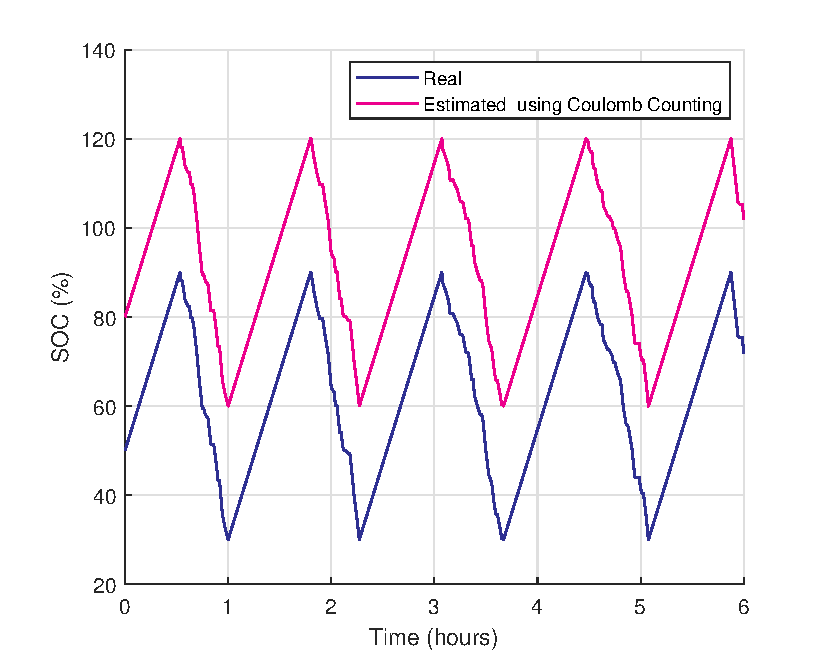
\includegraphics[width=\textwidth]{figs/Samuel/Figures/plotsbattest (1) (cropped) (pdfresizer.com).pdf}
        \caption{Estimate using Coulomb counting.}
        \label{fig:coolomb}
    \end{subfigure}
    \hspace{0\textwidth}
    \begin{subfigure}[b]{0.49\textwidth} % Use [b] to align captions at the bottom
        \centering
        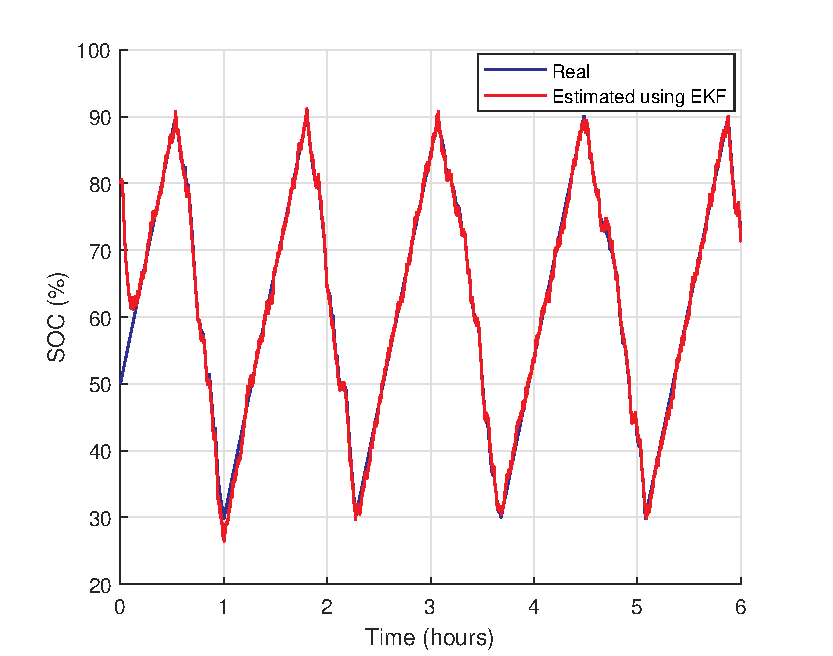
\includegraphics[width=\textwidth]{figs/Samuel/Figures/plotsbattest (1) (cropped) (pdfresizer.com) (1).pdf}
        \caption{Estimate additionally using \gls{ekf}.}
        \label{fig:kalmeff}
    \end{subfigure}
    \caption[Comparison of State of Charge Estimates]{Comparison of State of Charge estimates using the Simscape Kalman Filter Template}
    \label{fig:bmsestimefk}
\end{figure}

\subsection{Internal System}

The overall structure of the \acrshort{bms} is shown in Figure \ref{fig:bms_layout}, adapted from \cite{7555475}. For clarity, the battery pack depicts one set of the \acrshort{6s} cells. In reality, the system has a \acrshort{6s3p} configuration of cells. Sensor information from each cell in the battery pack is transmitted to the State Estimator, where Kalman filtering techniques are used to infer the states from the measurements. The State Estimator, including the \gls{ekf}, was incorporated into the model in MATLAB and Simulink utilising the Simscape Battery Toolbox.

The Master Control Unit represents the \textbf{STM32F405} microcontroller chosen in Section \ref{microcon}. The microcontroller implements the \gls{resc} switching techniques detailed in Section \ref{swit}, as depicted by the \textbf{Cell Equalisation} component of the BMS.

\begin{figure}[H]
  \centering
  \vspace{5mm}
  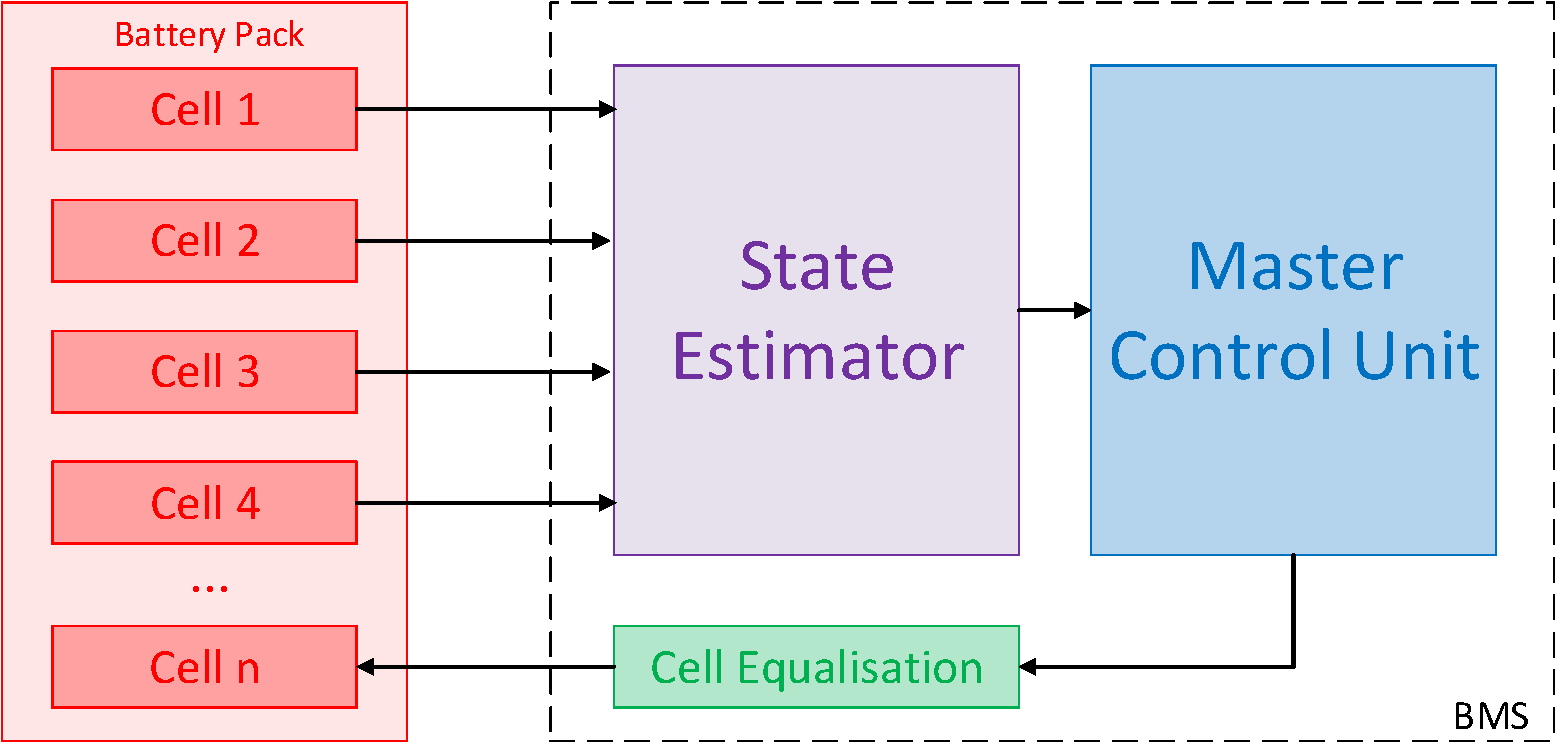
\includegraphics[width=0.75\textwidth]{figs/Samuel/Figures/BMS Internal (1)-cropped.pdf}
  \caption[Battery Management System Layout]{Battery Management System Layout adapted from \cite{7555475}}
  \label{fig:bms_layout}
  \vspace{5mm}
\end{figure}






\subsubsection{Battery Cell Stack Configuration}

A simplified diagram of the cell switching layout used is shown in Figure \ref{fig:bcs}. The switching topology used is the \gls{resc} layout. For conciseness, Figure \ref{fig:bcs} shows a simplified \gls{6s} circuit. In reality, a \gls{6s3p} layout is used, but this change does not affect the principles of operation. 

The use of capacitors, inductors and resistors allows for reduced equalisation time and less energy loss compared to simpler switched-capacitor methods \cite{8467638}. The core ideas and theory used to develop the \gls{resc} layout shown in Figure \ref{fig:bcs} are discussed in \cite{8681672}, and additional simulation and modelling are utilised to verify the configuration's applicability in this context.

\begin{figure}[H]
\centering
\vspace{10mm}
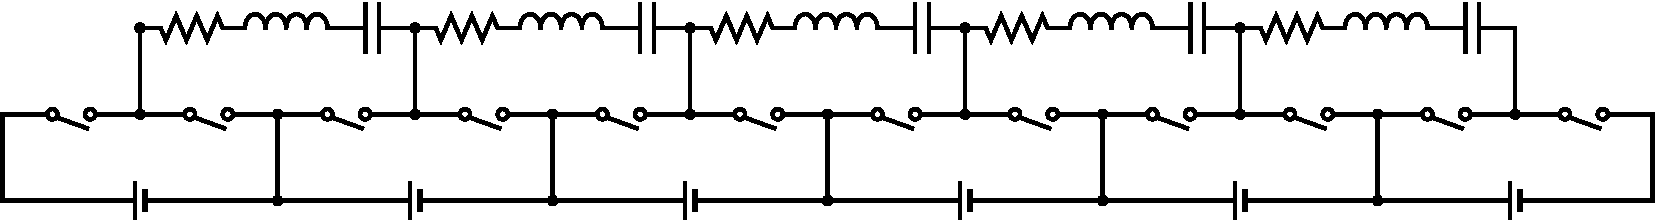
\includegraphics[width=0.99\textwidth]{figs/Samuel/Figures/resc1-cropped.pdf}
\caption[Simplified Battery Cell Stack Configuration]{Simplified battery cell stack configuration, adapted from \cite{8467638}}
\label{fig:bcs}
\end{figure}

\subsubsection{Cell Switching Simulations}
\label{swit}

The \gls{resc} switching technique outlined in \cite{8467638} was implemented in MATLAB, and the results obtained are shown in Figure \ref{fig:resccrop}. The methodology involved initialising each battery voltage with a random value between 3 V and 4 V and then performing the equalisation strategy. Figure \ref{fig:reccrop} shows the results obtained when using a simpler switched capacitor equalisation strategy. By contrasting the two plots shown in Figure \ref{fig:rescvrec}, the improved equalisation time given by the \gls{resc} strategy can be observed. 

The results produced by the simulation are consistent with results from similar models \cite{8467638}, albeit for cells with significantly different parameters. The moderate differences in cell voltages model a situation where a cell is damaged or unusable and, due to the cell stack configuration, normal operation can be quickly resumed by equalising the remaining cells.

\begin{figure}[H]
    \centering
    \vspace{5mm}
    \begin{subfigure}[b]{0.4\textwidth} % Use [b] to align captions at the bottom
        \centering
        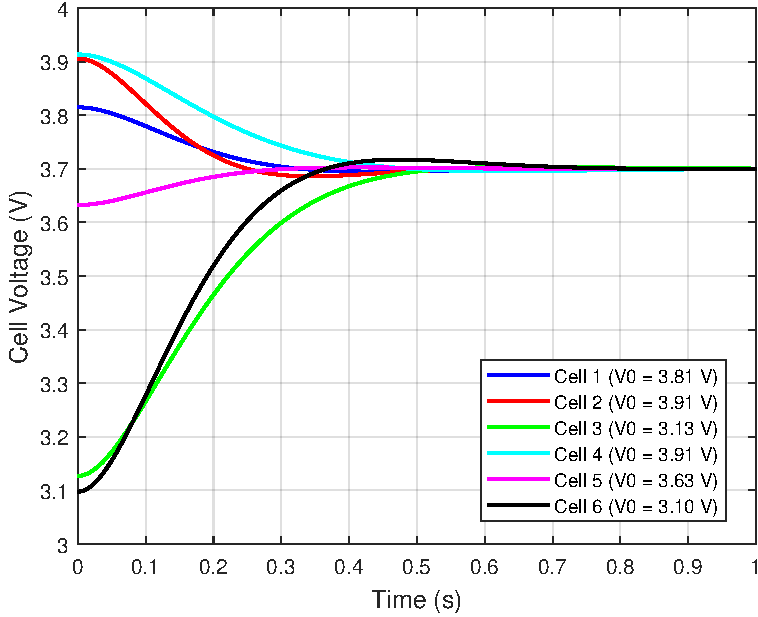
\includegraphics[width=\textwidth]{figs/Samuel/Figures/cellV-cropped.pdf}
        \caption{\gls{resc} switching strategy}
        \label{fig:resccrop}
    \end{subfigure}
    \hspace{0.07\textwidth}
    \begin{subfigure}[b]{0.388\textwidth} % Use [b] to align captions at the bottom
        \centering
        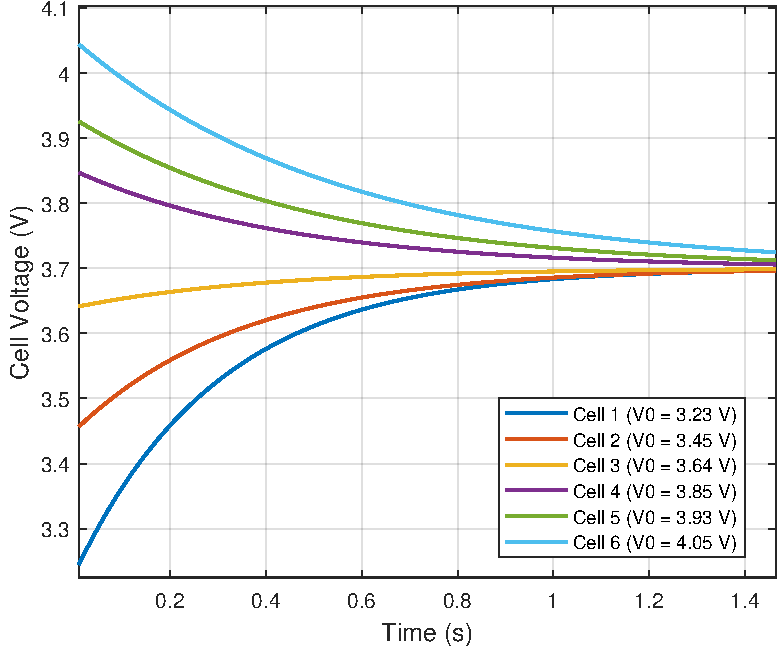
\includegraphics[width=\textwidth]{figs/Samuel/Figures/recpdf-cropped.pdf}
        \caption{Simpler switched-capacitor strategy}
        \label{fig:reccrop}
    \end{subfigure}
    \caption[Comparison of Cell Equalisation Strategies]{Comparison of cell equalisation strategies using the method outlined in \cite{8467638}}
    \label{fig:rescvrec}
\end{figure}

\subsubsection{Thermal Management Design and Simulations}

Designing an efficient thermal management system has numerous advantages for battery operation, with the most significant benefit being the ability to extend the cells' lifetimes by 30-50\% \cite{TOGUN20251077}. The design used in this \gls{bms} focuses on utilising passive cooling techniques to regulate and balance the battery's temperature. Specifically, \gls{tim} are used to regulate the transfer of heat between individual cells and their surroundings. In this design, a thin thermally conductive layer is inserted between the cells to aid heat dissipation. This passive cooling measure is especially useful when there are many cells, ensuring that even if some cells generate more heat, the overall temperature distribution remains balanced. Figure \ref{fig:tempythings} shows how temperature influences the discharge time (Figure \ref{fig:tempy1} from Chen, 2013 \cite{chen2013heat}) and the cycle life (Figure \ref{fig:tempy2} from \cite{REZVANIZANIANI2014110}). These graphs illustrate the importance of effective thermal management. Maintaining an operating temperature within the 20$^\circ\text{C}$ to 45$^\circ\text{C}$ range prevents the cell from discharging too rapidly and maximises the cycle life.

\begin{figure}[H]
    \centering
    \begin{subfigure}[b]{0.47\textwidth} % Use [b] to align captions at the bottom
        \centering
        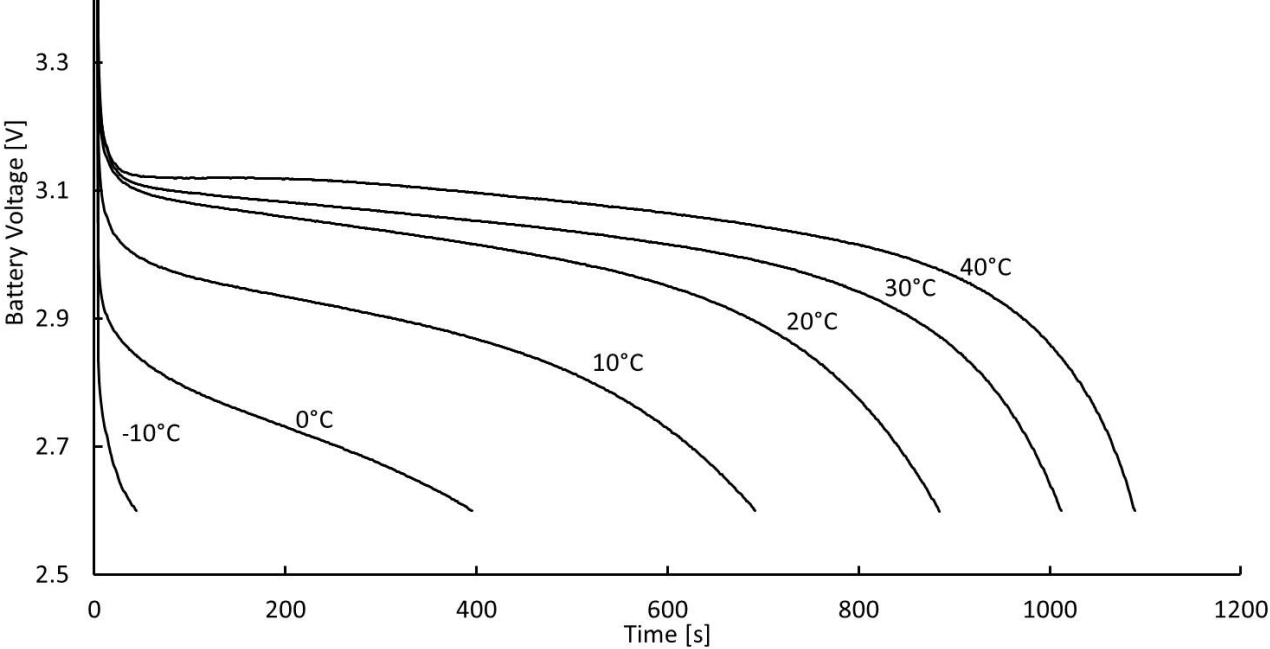
\includegraphics[width=\textwidth]{figs/Samuel/Figures/chenbattery.png}
        \caption{Cell discharge curves for varying temperatures \cite{chen2013heat}}
        \label{fig:tempy1}
    \end{subfigure}
    \hspace{0.04\textwidth}
    \begin{subfigure}[b]{0.47
    \textwidth} % Use [b] to align captions at the bottom
        \centering
        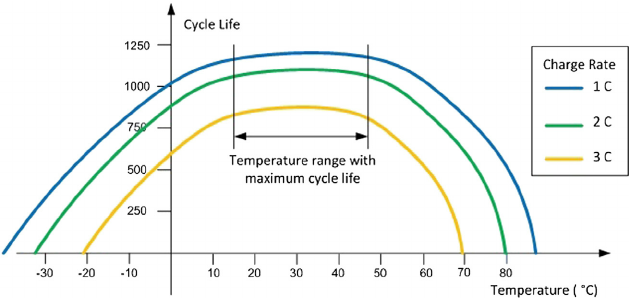
\includegraphics[width=\textwidth]{figs/Samuel/Figures/Lithium-ion-battery-life-vs-temperature-and-charging-rate-36-39-44-45.png}
        \caption{Variation of cycle life vs. temperature \cite{REZVANIZANIANI2014110}}
        \label{fig:tempy2}
    \end{subfigure}
    \caption[Effects of Temperature Variation on Cell Properties]{Effects of temperature variation on cell properties, figures from \cite{chen2013heat} (a) and \cite{REZVANIZANIANI2014110} (b).}
    \label{fig:tempythings}
\end{figure}

Using the Simulink and Simscape software, a high-fidelity model of the cells with the passive thermal management system was constructed. Cooling analysis of the battery was performed using simulation data, allowing for the use of realistic heat fluxes. The cell geometries were modelled, and the \gls{fem} was utilised to analyse the heat evolution over time by adapting an existing Simulink template.\footnote{\hyperlink{https://mathworks.com/help/pde/ug/battery-module-cooling-analysis-and-reduced-order-thermal-model.html}{mathworks.com/help/pde/ug/battery-module-cooling-analysis-and-reduced-order-thermal-model.html}} To provide meaningful results, the thermal analysis was run in parallel with the simulation example performed in Section \ref{mocs}. The battery temperature data shown in Figure \ref{fig:battemp} is an average of all 18 cells' temperatures for Agent 2 in the simulation. The graph shows that the temperature remains within the optimal temperature regime for the duration of the mission, indicating that the passive thermal management approach is sufficient to maximise cell performance and cycle life.

\begin{figure}[H]
\centering
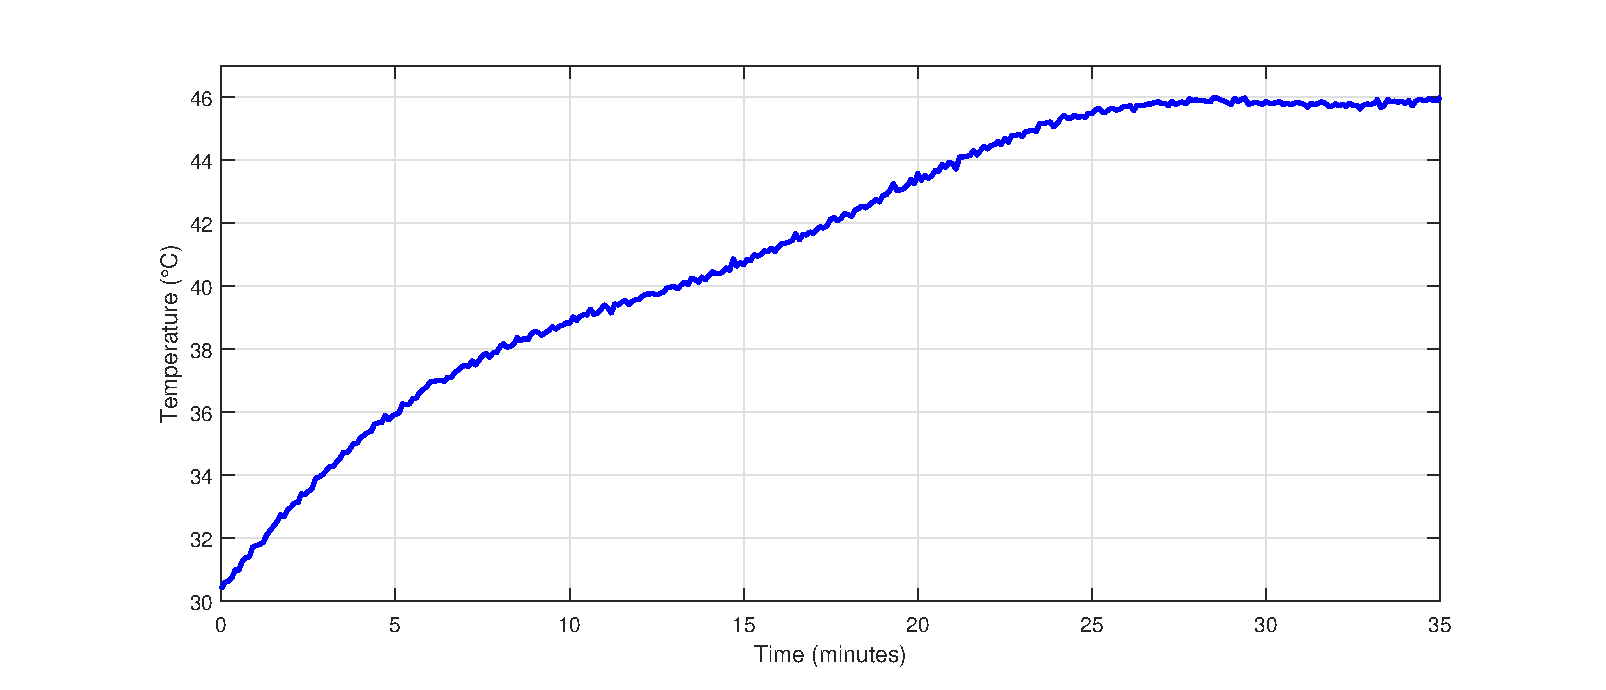
\includegraphics[width=0.73\textwidth]{figs/Samuel/Figures/batttemp.eps}
\caption{Battery temperature for Agent 2 in Section \ref{simdata}}
\label{fig:battemp}
\end{figure}

\subsection{DC-DC Converter Design}

A \acrshort{dcdc} converter is an integral part of the interface between the drone's battery management system and the rest of the \acrshort{uav}'s circuitry. It allows for the conversion of the cells' combined output voltage into a voltage which can be used in the drone's motors and control unit. Despite linear voltage regulation being a much simpler approach, switched-mode \acrshort{dcdc} converters are considered here because switched-mode converters have a much higher efficiency than linear regulators \cite{rogers2024powerelectronics}. As a result, fewer cells are required, thus reducing the drone's weight.

\subsubsection{Circuit Topology Selection}

Numerous switched-mode converter topologies exist, with the most common types being the Buck, Boost and Buck-Boost converters. For this application, however, a \textbf{non-isolated Ćuk converter} will be used. The crucial advantage gained by using a non-isolated Ćuk converter is the significantly reduced current ripple it exhibits compared to the other switched-mode converters mentioned \cite{cuk1981dc-to-dc}. The low current ripple minimises electrical noise within the circuit, which is important for ensuring that the data generated by the sensors is accurate. Another advantage of the Ćuk converter is that since there is continuous power transfer via the capacitor, electromagnetic interference is minimised, again helping to maximise the accuracy of the sensors. The most significant issue involved with using a Ćuk converter is the large voltage stress on the transistor \cite{Bailey:1641409}. This problem can be mitigated by selecting a \gls{mosfet} switch with a high voltage rating. In this instance, the battery's maximum output voltage is 25 V, so a \gls{mosfet} rated at 60 V gives an acceptable safety margin.

\subsubsection{Component Selection}

The Ćuk converter produces an inverted voltage output, so the corresponding circuitry must be carefully designed to account for the reversed polarity to ensure that the voltage does not require further inversion. Equation \ref{eq:cuk} gives the output voltage $V_{OUT}$ in terms of the input voltage $V_{IN}$ and the duty cycle $D$.

\begin{equation}
  \frac{V_{OUT}}{V_{IN}} = - \frac{D}{1-D}
  \label{eq:cuk}
\end{equation}

The layout of the non-isolated Ćuk converter circuit is shown in Figure \ref{fig:cukdiagram}.

\begin{figure}[H]
  \centering
  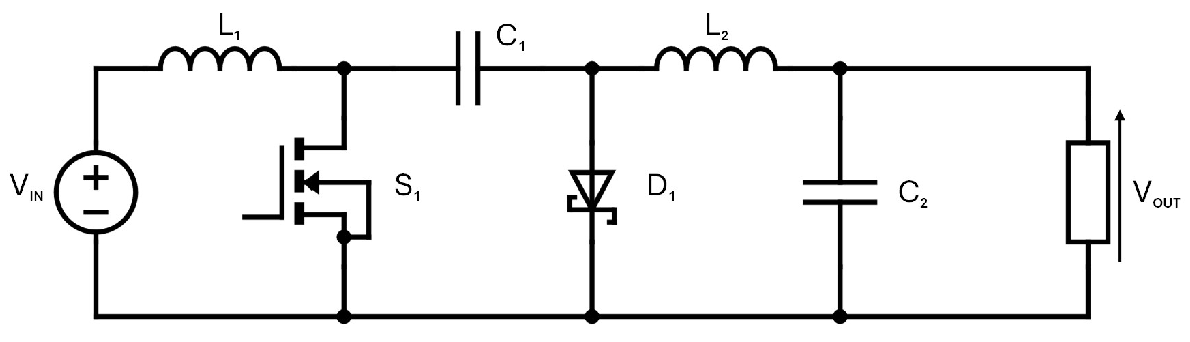
\includegraphics[width=0.68\textwidth]{figs/Samuel/Figures/mosfet cuk (1).pdf}
  \caption{Ćuk Converter Circuit Topology}
  \label{fig:cukdiagram}
\end{figure}



The switch S\textsubscript{1} in Figure \ref{fig:cukdiagram} operates at a \textbf{low switching frequency} $f_{sw} =$ 100 kHz. Using this low frequency minimises the potential for electromagnetic interference. The switching of the \acrshort{mosfet} is controlled by a gate driver. The diode D\textsubscript{1} shown in Figure \ref{eq:cuk} is a \textbf{Schottky diode}, which is designed for faster switching rates than a silicon p-n diode \cite{Schottky}. The battery will initially output 25 V when fully charged, with this decreasing to 18 V when the battery is in its discharged state. The passive component values for the Ćuk converter are determined by assuming that $V_{IN}$ = 21.5 V, which is the midpoint of the battery's output voltage range. The input and output current ripple must be sufficiently small to minimise noise, so the peak-to-peak inductor ripple currents $\Delta I_{L1}$ and $\Delta I_{L2}$ must satisfy $\Delta I_{L_{i}} \approx 0.1$ A,$\quad \text{for } i = 1, 2$. Also, the peak-to-peak output voltage ripple, $\Delta V_{OUT}$, should be approximately equal to 0.1\% of the output voltage, so for a 5 V output rail,  $\Delta V_{OUT} \approx $ 5 mV is required. The approximate output ripple currents and output voltage ripple are given by Equations \ref{eq:iL} and \ref{eq:Vo}, respectively \cite{EricksonRobertW2020FoPE}.

\begin{equation}
\Delta I_{L_{i}} \approx \frac{ V_{IN} D}{ f_{sw} L_i}, \quad \text{for } i = 1, 2
\label{eq:iL}
\end{equation}

\begin{equation}
\Delta V_{OUT} \approx \frac{V_{OUT} (1 - D)}{8C_2 L_2 (f_{sw})^2}
\label{eq:Vo}
\end{equation}


Equation \ref{eq:cuk} gives a duty cycle of $D \approx$ 0.19 for the given $V_{IN}$ and $V_{OUT}$ voltages. Using this duty cycle and rearranging Equation \ref{eq:iL} gives L\textsubscript{1} $\approx$ 400 $\mu$H and L\textsubscript{2} $\approx$ 400 $\mu$H, since both inductors have the same maximum current ripple. Rearranging Equation \ref{eq:Vo} gives C\textsubscript{2} $\approx$ 20 $\mu$F, which ensures that $V_{OUT}$ is smooth. C\textsubscript{1} $\approx$ 40 $\mu$F is selected to balance the benefits of a low equivalent series resistance with the added smoothness gained from a higher capacitance value.  The component values are chosen from the \acrshort{bs} 2488 E24 series preferred values \cite{HLT}, so: C\textsubscript{1} $=$ 43 $\mu$F, L\textsubscript{1} $=$ 390 $\mu$H, C\textsubscript{2} $=$ 20 $\mu$F and  L\textsubscript{2} $=$ 390 $\mu$H. 

\subsubsection{Circuit Simulation}

The Ćuk converter is accurately modelled in a simulation environment to verify the expected behaviour of the \acrshort{dcdc} converter over the range of $V_{IN}$ values supplied from the battery management system. The Simscape Electrical Ćuk converter template from MathWorks is used to implement the model of the circuit, using the ode23tb differential equation solver to compute the voltage and current evolutions over time. The ode23tb equation solver is an implicit Runge-Kutta method \cite{matlab_ode23tb}, which is able to solve the Ćuk converter equations both rapidly and accurately.

Modelling the \gls{esr} of each component is an important aspect of the simulation since the \acrshort{esr} has a significant impact on the output voltage ripple $\Delta V_{OUT}$ and output current ripple $\Delta I_{OUT}$. The Simscape Electrical software can model the \acrshort{esr}, so the numerical values for the \acrshort{esr} of the components were included in the simulation. To validate the theoretical output voltage ripple and current ripple across all of the possible battery output voltages, the simulation was run for input voltage values at 1 V intervals within the operating range of the battery, $V_{IN}$ = 18 V to $V_{IN}$ = 25.2 V. The results of these simulations are shown in Table \ref{tab:converter_performance}.

\begin{table}[h]
    \centering
    \renewcommand{\arraystretch}{1.2}
    \begin{tabular}{cccc}
        \toprule
        $V_{IN}$ (V) & $\Delta V_{OUT}$ (mV) & $\Delta I_{OUT}$ (A) & $D$ \\
        \midrule
        18.0 & 5.27 & 0.100 & 0.217 \\
        19.0 & 5.13 & 0.098 & 0.208 \\
        20.0 & 5.41 & 0.103 & 0.200 \\
        21.0 & 5.63 & 0.103 & 0.192 \\
        22.0 & 5.52 & 0.105 & 0.185 \\
        23.0 & 5.53 & 0.102 & 0.179 \\
        24.0 & 5.63 & 0.105 & 0.172 \\
        25.0 & 5.67 & 0.106 & 0.167 \\
        25.2 & 5.63 & 0.106 & 0.166 \\
        \bottomrule
    \end{tabular}
    \caption{Output Ripple Characteristics and Duty Cycle Relationship}
    \label{tab:converter_performance}
\end{table}


 The results conform with the theoretical expectations, in most cases having similar numerical values to those predicted by Equations \ref{eq:iL} and \ref{eq:Vo}. Any discrepancies from the predicted values are likely due to second-order effects included in the simulation that Equations \ref{eq:iL} and \ref{eq:Vo} do not model. The simulation shows that the output voltage ripple and current ripple are well within the acceptable range for low-noise applications. Therefore, the Ćuk converter can safely be deployed as part of the \acrshort{bms} circuitry onboard the drone, with minimal electromagnetic interference.


For each of the voltages tested in Table \ref{tab:converter_performance} above, two plots of the output voltage $V_{OUT}$ and output current $I_{OUT}$ were generated. As an example, the results produced with $V_{IN}$ = 22 V are shown in Figure \ref{fig:cukmatlab}. In each of the plots, the average value is shown by a black dashed line, and labelled vertical lines denote the \textit{peak-to-peak} voltage and current ripple on the waveforms in Figures \ref{fig:cukmatlab_a} and \ref{fig:cukmatlab_b}, respectively. 

\begin{figure}[H]
\centering
\subfloat[Plot of the steady-state output voltage $V_{OUT}$]{
    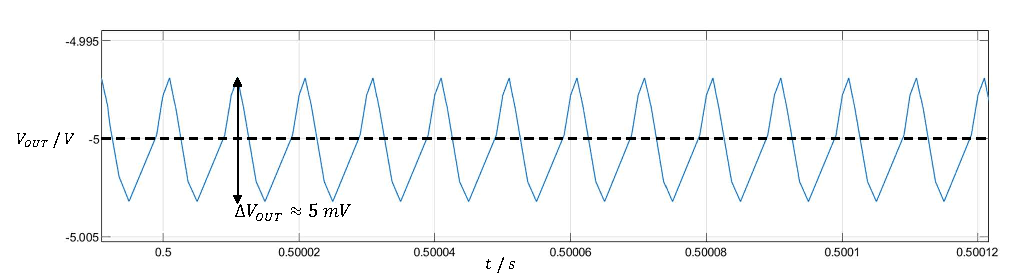
\includegraphics[width=\textwidth]{figs/Samuel/Figures/CukPlots (cropped) (pdfresizer.com).pdf}
    \label{fig:cukmatlab_a}
}

\vspace{0.1cm} % Add vertical space between subfigures (adjust as needed)

\subfloat[Plot of the steady-state output current $I_{OUT}$]{
    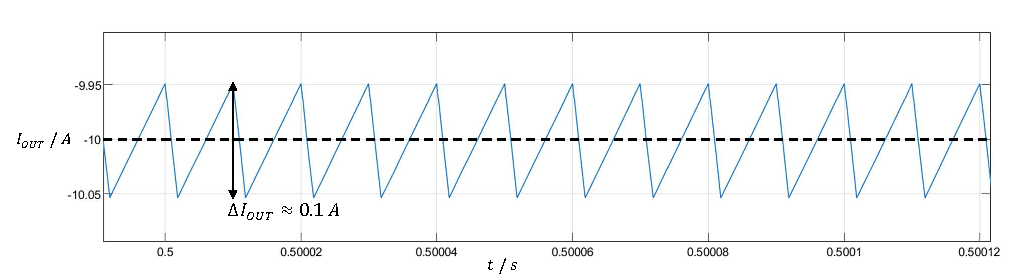
\includegraphics[width=\textwidth]{figs/Samuel/Figures/CukPlots (cropped) (pdfresizer.com) (1).pdf}
    \label{fig:cukmatlab_b}
}
\caption{Simscape simulation results for the Ćuk converter}
\label{fig:cukmatlab}
\end{figure}

\subsection{Overall Circuit Layout}

A high-fidelity simulation of the \gls{bms} was constructed using MATLAB, Simulink and Simscape. This model was then integrated into the overall system to allow the multi-agent system to be modelled using the designed \gls{bms}; the results obtained are shown in Section \ref{mocs}. Figure \ref{fig:bms_ovrlayout} shows a simplified version of the \gls{bms} location within the drone's circuitry, as modelled in the simulation.

\begin{figure}[H]
  \centering
  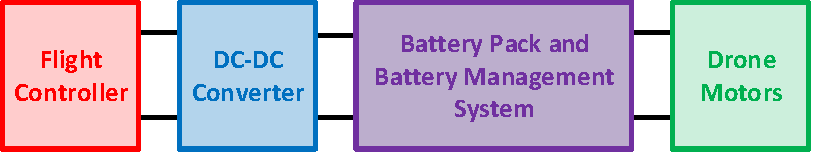
\includegraphics[width=0.79\textwidth]{figs/Samuel/Figures/BMS-cropped.pdf}
  \caption{Overall circuitry layout}
  \label{fig:bms_ovrlayout}
\end{figure}

